
% File ucca_parsing.tex
%

\documentclass[11pt]{article}
\usepackage{colacl-onecolumn}
\usepackage{times}
\usepackage{url}
\usepackage{amsmath}
\usepackage{breqn}
\usepackage{latexsym}
\usepackage{pgfplotstable}
\usepackage{algorithm2e}
\usepackage{hhline}
\usepackage{multirow}
\usepackage[font=small]{caption}
\usepackage{subcaption}
\usepackage{hyperref}
\usepackage{color}
\usepackage{lipsum,adjustbox}
\usepackage{tikz}
\usepackage{tikz-dependency}
\usepackage{rotating}
\usepackage{float}
\usetikzlibrary{shapes,fit,calc,er,positioning,intersections,decorations.shapes,mindmap,trees}
\tikzset{decorate sep/.style 2 args={decorate,decoration={shape backgrounds,shape=circle,
      shape size=#1,shape sep=#2}}}

\flushbottom \onecolumn

\newcommand{\com}[1]{}
\newcommand{\secref}[1]{Section~\ref{#1}}
\newcommand{\figref}[1]{Figure~\ref{#1}}
\newcommand{\tabref}[1]{Table~\ref{#1}}
\DeclareMathOperator*{\argmin}{argmin}
\DeclareMathOperator*{\argmax}{argmax}
\SetKwRepeat{Do}{do}{while}
\renewcommand\AlCapFnt{\normalfont\small}

\makeatletter
\renewcommand{\paragraph}{
  \@startsection{paragraph}{4}
  {\z@}{.5ex \@plus .5ex \@minus .2ex}{-1em}
  {\normalfont\normalsize\bfseries}
}
\makeatother

\newcommand\BibTeX{B\textsc{ib}\TeX}

\title{HUME: Human UCCA-Based Evaluation of Machine Translation \\
  Supplementary Matrerial}


\begin{document}
\maketitle

\section{Another Example of HUME Annotation}

Sample UCCA annotation of a source sentence, translation (below in italics), 
and translation judgements over the source units, marked with A,B,R,O,G labels. Yellow/blue marks nodes annotated with A/B, respectively.
In the experiments reported in the paper,
the translation is in German, Romaninan, Polish or Czech.
``became a passion'' is marked as atomic, as it is a multi-word expression.
The dashed line indicates that ``she'' is also a child of the unit ``greatly improved''.
UCCA categories, and alignment between source and translation are omitted for brevity.


\begin{figure*}[h]
  \begin{adjustbox}{trim=2.3cm 0 0 0}
   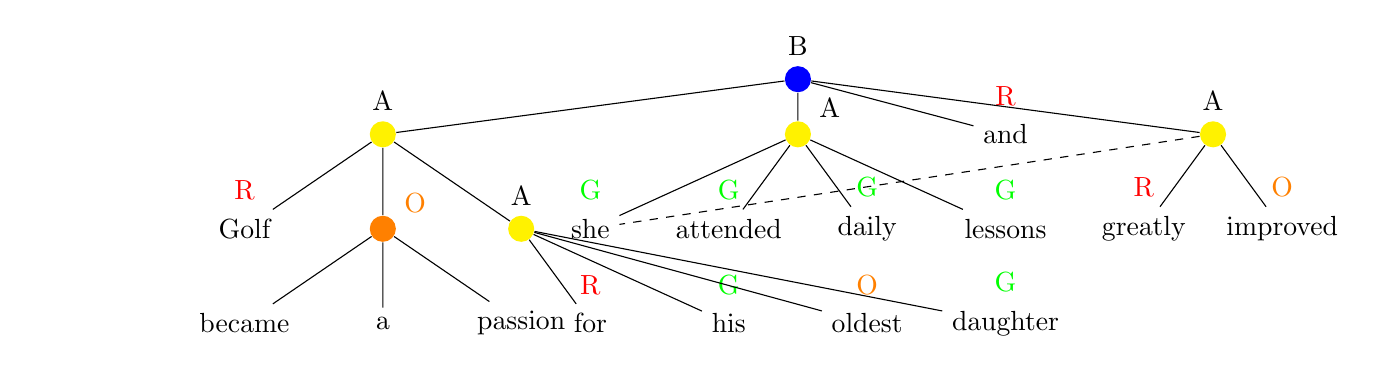
\begin{tikzpicture}
     [ level distance=12mm,
	   level 1/.style={sibling distance=7.5em,level distance=7mm},
       level 2/.style={sibling distance=5em,level distance=12mm},
       level 3/.style={sibling distance=5em},
       level 4/.style={sibling distance=3em}]
     %[semithick, x=2.4cm,y=0.8cm, >=latex, baseline=7ex,
     %  inner sep=.3ex, outer sep=.7ex, minimum size=1.2ex,->]
   \node (ROOT) [label={B}] [fill=blue, circle] {}
   child {node (H3) [label={A}] [fill=yellow,circle] {}
     child {node [label={[red]:R}] {Golf} edge from parent node[left] {}}
     child {node (H1) [label={[orange]30:O}] [fill=orange,circle] {}
       child {node [label={}] {became} edge from parent node[left]  {}}
       child {node [label={}] {a} edge from parent node[left]  {}}
       child {node [label={}] {passion} edge from parent node[left]  {}}
     }
     child {node (H2) [label={A}] [fill=yellow,circle] {}
       child {node {} edge from parent[draw=none] {}}
       child {node {} edge from parent[draw=none] {}}
       child {node {} edge from parent[draw=none] {}}
       child {node {} edge from parent[draw=none] {}}
       child {node [label={[red]:R}] {for} edge from parent node[left]  {}}
       child {node [label={[green]:G}] {his} edge from parent node[left]  {}}
       child {node [label={[orange]:O}] {oldest} edge from parent node[left]  {}}
       child {node [label={[green]:G}] {daughter} edge from parent node[left]  {}}
     }
   }
   child {node {} edge from parent[draw=none] {}}
   child {node (H4) [label={[]30:A}] [fill=yellow,circle] {}
     child {node (she) [label={[green]:G}] {she} edge from parent node[left]  {}}
     child {node [label={[green]:G}] {attended} edge from parent node[left]  {}}
     child {node [label={[green]:G}] {daily} edge from parent node[left]  {}}
     child {node [label={[green]:G}] {lessons} edge from parent node[left]  {}}
   }
   child {node [label={[red]:R}] {and} edge from parent node[left]  {}}
   child {node (H5) [label={A}] [fill=yellow,circle] {}  
     child {node [label={[red]:R}] {greatly} edge from parent node[left] {}}
     child {node [label={[orange]:O}] {improved} edge from parent node[left] {}}
   };
   \draw[dashed] (H5) -> (she) ;
   \end{tikzpicture}
   \\
  \end{adjustbox}
    % Ondrej removed the width=\textwidth from the options below to keep font
	% unenlarged:
  \adjustbox{center,margin=.5em}{\it His old daughter loved tennis, and took daily lessons however good he was}


  \label{fig:hume_tree}
 
\end{figure*}





\end{document}
